\subsection{Product perspective}
\subsubsection{Class diagrams}
The following pages present the class diagrams which give an overall description of the main elements through the use of a conceptual model. Only the relevant parts of the system are present for the sake of clarity.
\begin{sidewaysfigure}
\centering
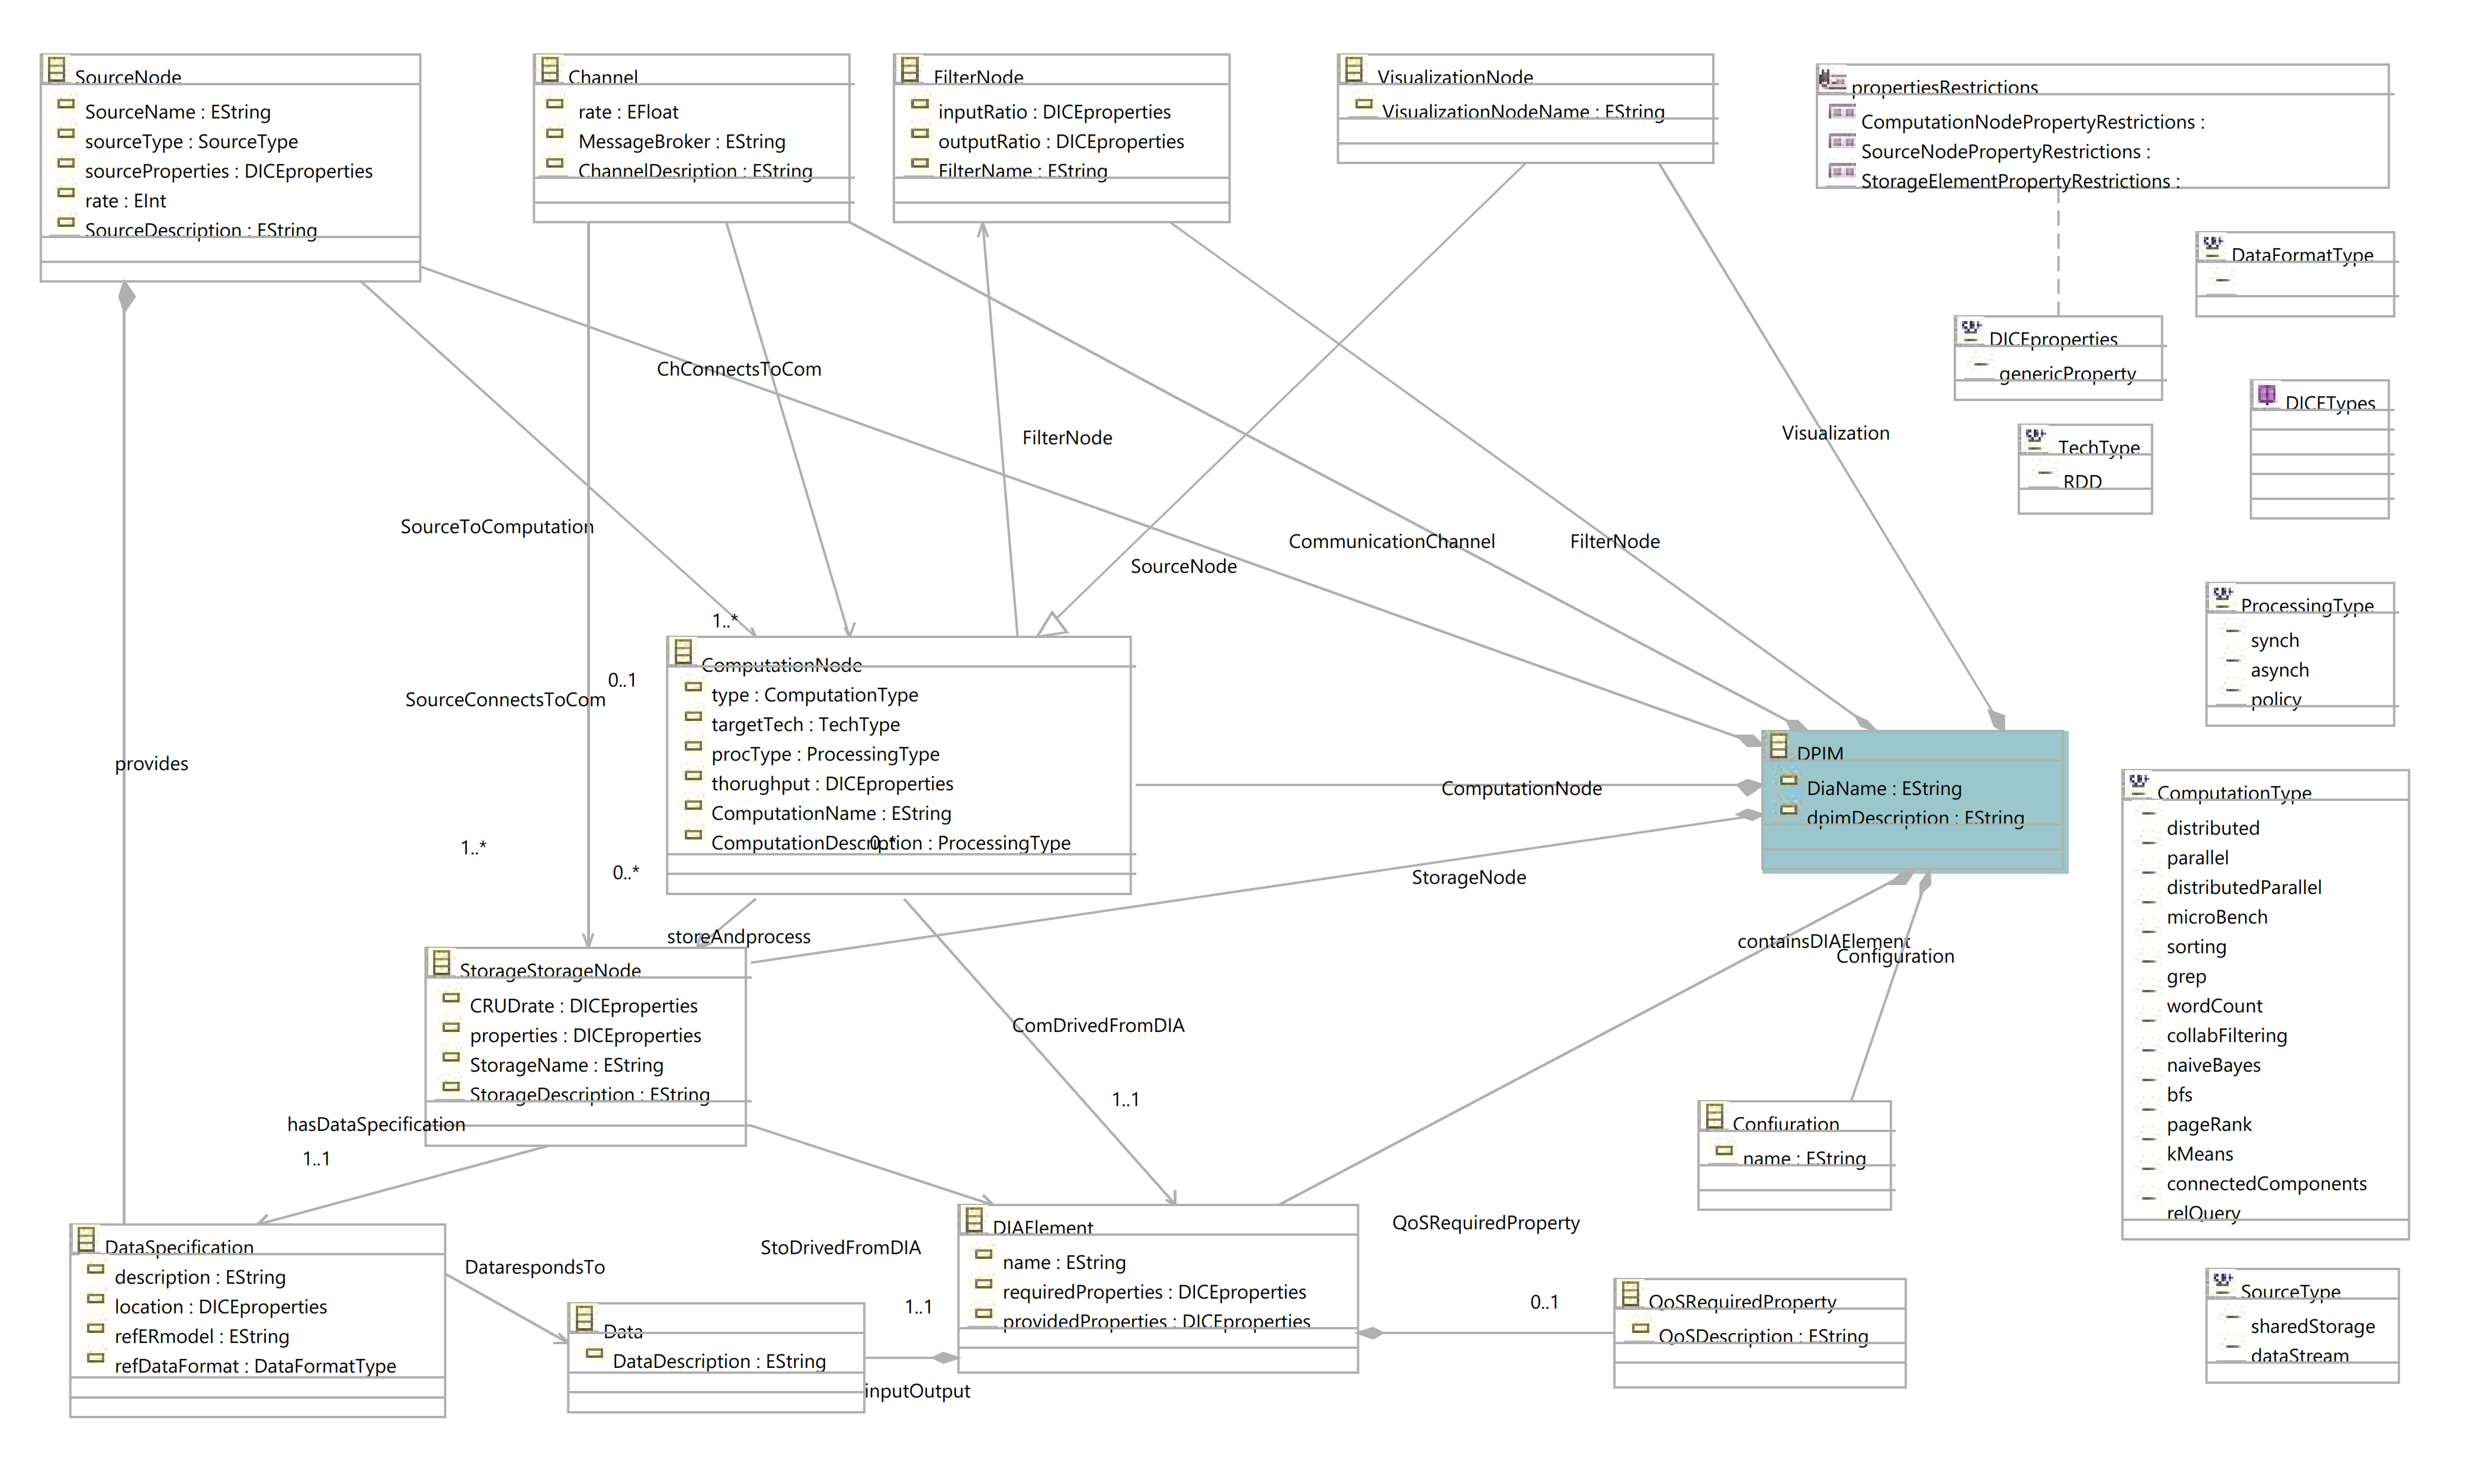
\includegraphics[width=\textwidth]{Images/11.png}
\caption{\label{fig:metamodel}DICE DPIM metamodel.}
\end{sidewaysfigure}

\newpage
\subsubsection{State machine diagrams}
{\todo
The evolution of the states for of the system is visualized using the state machine UML model.

    \begin{figure}[H]
        %\includegraphics[width=\linewidth]{rasd_statemachine_grpreq.jpg}
        \caption{Statechart of a request for a group of cutsomers data}
        \label{fig:statemachine_grpreq}
    \end{figure}

    \begin{figure}[H]
        %\includegraphics[width=\linewidth]{rasd_statemachine_specreq.jpg}
        \caption{Statechart of a request for a single cutsomer's data}
        \label{fig:statemachine_specreq}
    \end{figure}

    \begin{figure}[H]
        %\includegraphics[width=\linewidth]{rasd_statemachine_runevent.jpg}
        \caption{Statechart of a running event}
        \label{fig:statemachine_runevent}
    \end{figure}
}


\subsection{Product functions}
{
    \todo
    \noindent\emph{CLup} [...]
\\Let's see more in the details the functions mentioned above:
}

\paragraph{Basic User functions} These functions are available to all Users:
\begin{itemize}
    \item \textbf{Registration and Login}\\
    \emph{CLup} must be able to recognize Users between requests, to display correct information and as means of authentication. Therefore, Users should be able to create a personal account through the App. After creating an account, Users should login to access the functions described in the following paragraphs;
    \item \textbf{Obtaining a Ticket}\\
    \emph{CLup} has a waiting list of the users who are currently waiting to enter the Shop. Registered Users are able to join the list via the App, thus obtaining an estimate of the waiting time. This operation is certified by a Ticket. Notifications can be sent to the Users' devices to remind them when it is their turn to enter the Store;
    \item\textbf{Booking a visit}\\
    \emph{CLup} allows Users to book a visit to the Shop for a specific date in the future, via the App. This operation is finalized by the emission of a Booking. This data is used to determine whether the next bookings should be accepted, in order to prevent congestion in the Shop;
    \item\textbf{Specifying item categories}\\
    Furthermore, Users can specify categories of products they intend to buy, when obtaining both a Ticket and a Booking.This makes possible to better optimize the capacity of the departments of the Shop.
    \end{itemize}
    
\paragraph{Third Parties base functions}
    These functions should be accessible to the clerks of the Third Party, since they are required for the proper working of the system, at an operational level:
\begin{itemize}
    \item\textbf{Substitute ticket distribution}\\
    Third Parties shall be able to generate a ticket for Users who do not have the required technologies, which allows them to join the waiting list. Booking is only allowed via the App, since it requires more detailed information;
    \item\textbf{Ticket and Booking validation}\\
    \emph{CLup} allows Third Parties to check Users' tickets against those stored in the system. This is fundamental to deny forged tickets.
\end{itemize}    
\paragraph{Third Parties administration functions}
These functions must only be accessible to the managers of the Third Party, since they control administrative aspects of the service, which handle sensible or critical data:
\begin{itemize}
    \item\textbf{Store creation and configuration}\\
    Third Parties shall be able to enlist their store in the \emph{CLup} system, specifiying opening hours and departments with the respective capacities. This is only possible with a manager account, while the clerks should only be allowed to;
    \item\textbf{Store occupancy checking}\\
    \emph{CLup} allows Third Parties to monitor entrances, to ensure all of the imposed restrictions are being followed. These data are also a source of useful insights for a business perspective.
\end{itemize}
\subsection{User characteristics}
\subsection{Assumptions, dependencies and constraints}
